\documentclass[aspectratio=169]{beamer}
\usetheme{Bruno}
\usepackage{amsmath}
\usepackage{siunitx}
\usepackage[american,RPvoltages]{circuitikz}
\ctikzset{capacitors/scale=0.7}
\usepackage{tabularx}
\newcolumntype{C}{>{\centering\arraybackslash}X}
\usepackage{tabu}
\usepackage[spanish]{babel}
\usepackage{booktabs}
\usepackage{pgfplots}
\usepgfplotslibrary{units, fillbetween} 
\pgfplotsset{compat=1.16}
\renewcommand\tabularxcolumn[1]{m{#1}}% for vertical centering text in X column
\usetikzlibrary{arrows, arrows.meta}
\ctikzset{capacitors/scale=0.7}
\title{Electricidad I: \\ \emph{Capacitores e Inductores}}
\usetikzlibrary{arrows, arrows.meta}
\author{
    Juan J. Rojas
}
\institute{Instituto Tecnológico de Costa Rica}
\date{\today}
\background{fig/background.jpg}
\begin{document}
\sisetup{unit-math-rm=\mathrm,math-rm=\mathrm} % change sinitx font
\sisetup{output-decimal-marker = {,}}
\maketitle

\begin{frame}{Capacitor}
    \begin{columns}[onlytextwidth]
    \begin{column}{0.6\textwidth}
        \textbf{Construcción:}\\
        Dos placas de un material conductor, separadas por un material dieléctrico.\\[8pt]
        \textbf{Principio:}\\
        Almacenamiento de energía en un campo eléctrico\\[8pt]
        \begin{tabularx}{\linewidth}{CC}
        \textbf{Ecuación} & \textbf{Símbolo}\\
        \begin{equation*}
            i = C\,\frac{dv}{dt}
        \end{equation*}
        &
        \begin{circuitikz}[scale=0.8]\draw
            (0,0)
                to[C,l=$C$,v=$v$, voltage shift=3, i=$i$, o-o]
            (3,0)
            ;
        \end{circuitikz} 
        \end{tabularx}
        \end{column}
    \begin{column}{0.4\textwidth}
    \begin{center}
        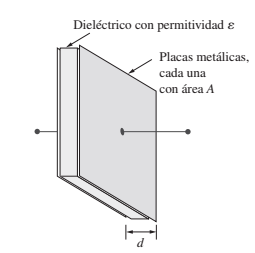
\includegraphics[scale=0.8]{fig/capacitor.png}
    \end{center}
    \flushright \cite{charles2013fundamentos}
\end{column}
\end{columns}
\end{frame}

\begin{frame}{Capacitancia}
    \begin{columns}[onlytextwidth]
    \begin{column}{0.6\textwidth}
        Es una medida de la oposición al cambio del voltaje en el capacitor.\\[6pt] 
        Unidad:\hspace{6pt}\emph{Farad},\hspace{6pt}$\si{\farad}\,[\si{\ampere\cdot\second\,\volt^{-1}}]$\\[6pt] 
        Depende de:
        \begin{equation*}
            C = \frac{\epsilon A}{d},
        \end{equation*}
        donde $\epsilon$ es la permitividad del material dieléctrico, $A$ es el area de las placas conductoras, y $d$ es la distancia entre las placas. 
    \end{column}
    \begin{column}{0.4\textwidth}
    \begin{center}
        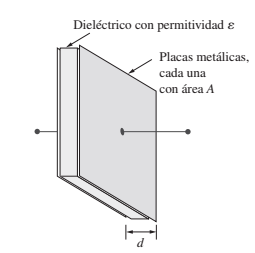
\includegraphics[scale=0.8]{fig/capacitor.png}
    \end{center}
    \flushright \cite{charles2013fundamentos}
\end{column}
\end{columns}
\end{frame}

\begin{frame}{Capacitor}
\begin{columns}[onlytextwidth]
    \begin{column}{0.75\textwidth}
        \begin{itemize}
            \setlength\itemsep{1em}
            \item Si $\frac{dv}{dt} = 0$, $i=0$; por lo tanto en corriente directa el capacitor se comporta como un abierto.
            \item Para que $\frac{dv}{dt}$ exista, el votaje no debe tener discontinuidades; por lo tanto un capacitor no permite cambios instantáneos en el voltaje.
            \item La corriente del capacitor puede cambiar de valor y/o dirección abruptamente. 
            \item Un capacitor ideal no disipa potencia, solo almacena y libera energía.
        \end{itemize}
    \end{column}
    \begin{column}{0.25\textwidth}
    \begin{center}
        \begin{circuitikz}[scale=0.8]\draw
            (0,0)
                to[C,l=$C$,v=$v$, voltage shift=3, i=$i$, o-o]
            (4,0)
            ;
        \end{circuitikz} 
        \begin{equation*}
            i = C\,\frac{dv}{dt}
        \end{equation*}
    \end{center}
    \end{column}
\end{columns}
\end{frame}

\begin{frame}{Capacitores en serie}
\begin{columns}[onlytextwidth]
    \begin{column}{0.5\textwidth}
    \begin{center}
        \begin{circuitikz} [scale=1]\draw
            (3,0)
                to[C,l=$C_3$,o-]
            (0,0)	
                to[C,l=$C_2$]
            (0,3)
                to[C,l=$C_1$,i^<=$i$,-o]
            (3,3)
            ;
        \end{circuitikz}
    \end{center}
    \end{column}
    \begin{column}{0.5\textwidth}
    \begin{center}
        Caso general:
        \begin{equation*}
            \frac{1}{C_{eq}}=\frac{1}{C_1}+\frac{1}{C_2}+\frac{1}{C_3}
        \end{equation*}
       Caso especial, solo dos capacitores:
        \begin{equation*}
            C_{eq}=\frac{C_1\cdot C_2}{C_1+ C_2}
        \end{equation*}
    \end{center}
    \end{column}
\end{columns}
\end{frame}

\begin{frame}{Capacitores en paralelo}
\begin{columns}[onlytextwidth]
    \begin{column}{0.5\textwidth}
    \begin{center}
        \begin{circuitikz} [scale=1]\draw
            (1,3)
                to[short,o-]
            (0,3)	
                to[C,l_=$C_3$]
            (0,0)
                to[short,-o]
            (1,0)
            (0,3) -- (-1.5,3)
                to[C,l_=$C_2$]
            (-1.5,0) -- (0,0)
            (-1.5,3) -- (-3,3)
                to[C,l_=$C_1$]
            (-3,0) -- (-1.5,0)
            (1,3)
                to[open,v^=$v$]
            (1,0)
            ;
        \end{circuitikz}
    \end{center}
    \end{column}
    \begin{column}{0.5\textwidth}
    \begin{center}
        \begin{equation*}
            C_{eq}=C_1+C_2+C_3
        \end{equation*}
    \end{center}
    \end{column}
\end{columns}
\end{frame}

\begin{frame}{Inductor}
    \begin{columns}[onlytextwidth]
    \begin{column}{0.6\textwidth}
        \textbf{Construcción:}\\
        Una bobina de alambre conductor, enrollada en un núcleo de un material ferromagnético.\\[8pt]
        \textbf{Principio:}\\
        Almacenamiento de energía en un campo magnético\\[8pt]
        \begin{tabularx}{\linewidth}{CC}
        \textbf{Ecuación} & \textbf{Símbolo}\\
        \begin{equation*}
            v = L\,\frac{di}{dt}
        \end{equation*}
        &
        \begin{circuitikz}[scale=0.8]\draw
            (0,0)
                to[L,l=$L$,v=$v$, voltage shift=3, i=$i$, o-o]
            (3,0)
            ;
        \end{circuitikz} 
        \end{tabularx}
        \end{column}
    \begin{column}{0.4\textwidth}
    \begin{center}
        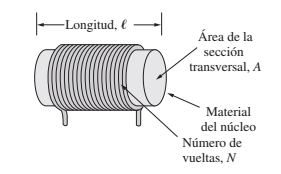
\includegraphics[scale=0.8]{fig/inductor.png}
    \end{center}
    \flushright \cite{charles2013fundamentos}
\end{column}
\end{columns}
\end{frame}

\begin{frame}{Inductancia}
    \begin{columns}[onlytextwidth]
    \begin{column}{0.6\textwidth}
        Es una medida de la oposición al cambio de la corriente en el inductor.\\[6pt]
        Unidad:\hspace{6pt}\emph{Henry},\hspace{6pt}\si{\henry}\,[\si{\volt\cdot \second\,\ampere^{-1}}]\\[6pt]
        Depende de:
        \begin{equation*}
            L = \frac{N\,^2 \mu A}{l},
        \end{equation*}
        donde $l$ es la longitud y $N$ es el número de vueltas del alambre conductor, $A$ es el área de sección trasversal y $\mu$ es la permeabilidad del material ferromagnético del núcleo. 
    \end{column}
    \begin{column}{0.4\textwidth}
    \begin{center}
        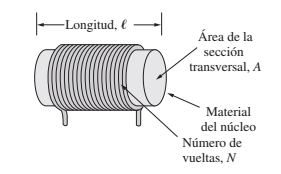
\includegraphics[scale=0.8]{fig/inductor.png}
    \end{center}
    \flushright \cite{charles2013fundamentos}
\end{column}
\end{columns}
\end{frame}

\begin{frame}{Inductor}
    \begin{columns}[onlytextwidth]
    \begin{column}{0.75\textwidth}
        \begin{itemize}
            \setlength\itemsep{1em}
            \item Si $\frac{di}{dt} = 0$, $v=0$; por lo tanto en corriente directa el inductor se comporta como un corto.
            \item Para que $\frac{di}{dt}$ exista, la corriente no debe tener discontinuidades; por lo tanto un inductor no permite cambios instantáneos en la corriente.
            \item El voltaje del inductor puede cambiar de valor y/o polaridad abruptamente. 
            \item Un inductor ideal no disipa potencia, solo almacena y libera energía.
        \end{itemize}
    \end{column}
    \begin{column}{0.25\textwidth}
    \begin{center}
        \begin{circuitikz}[scale=0.8]\draw
            (0,0)
                to[L,l=$L$,v=$v$, voltage shift=3, i=$i$, o-o]
            (4,0)
            ;
        \end{circuitikz} 
        \begin{equation*}
            v = L\,\frac{di}{dt}
        \end{equation*}
    \end{center}
\end{column}
\end{columns}
\end{frame}

\begin{frame}{Inductores en serie}
\begin{columns}[onlytextwidth]
    \begin{column}{0.5\textwidth}
    \begin{center}
        \begin{circuitikz} [scale=1]\draw
            (3,0)
                to[L,l=$L_3$,o-]
            (0,0)	
                to[L,l=$L_2$]
            (0,3)
                to[L,l=$L_1$,i^<=$i$,-o]
            (3,3)
            ;
        \end{circuitikz}
    \end{center}
    \end{column}
    \begin{column}{0.5\textwidth}
    \begin{center}
        \begin{equation*}
            L_{eq}=L_1+L_2+L_3
        \end{equation*}
    \end{center}
    \end{column}
\end{columns}
\end{frame}

\begin{frame}{Inductores en paralelo}
\begin{columns}[onlytextwidth]
    \begin{column}{0.5\textwidth}
    \begin{center}
        \begin{circuitikz} [scale=1]\draw
            (1,3)
                to[short,o-]
            (0,3)	
                to[L,l_=$L_3$]
            (0,0)
                to[short,-o]
            (1,0)
            (0,3) -- (-1.5,3)
                to[L,l_=$L_2$]
            (-1.5,0) -- (0,0)
            (-1.5,3) -- (-3,3)
                to[L,l_=$L_1$]
            (-3,0) -- (-1.5,0)
            (1,3)
                to[open,v^=$v$]
            (1,0)
            ;
        \end{circuitikz}
    \end{center}
    \end{column}
    \begin{column}{0.5\textwidth}
    \begin{center}
        Caso general:
        \begin{equation*}
            \frac{1}{L_{eq}}=\frac{1}{L_1}+\frac{1}{L_2}+\frac{1}{L_3}
        \end{equation*}
       Caso especial, solo dos inductores:
        \begin{equation*}
            L_{eq}=\frac{L_1\cdot L_2}{L_1+ L_2}
        \end{equation*}
    \end{center}
    \end{column}
\end{columns}
\end{frame}

\begin{frame}{Resumen}
    \begin{center}
        \begin{tabularx}{14cm}{C C C}
        \toprule
        Variable & Ecuación $v-i$ & Ecuación $i-v$ \\
        \midrule
       Capacitor & $v=\frac{1}{C}\int_{t_0}^{t} i(t)dt + v(t_0) $ & $i = C\,\frac{dv}{dt}$ \\[5pt]
        Inductor & $v = L\,\frac{di}{dt}$ & $i=\frac{1}{L}\int_{t_0}^{t} v(t)dt + i(t_0) $\\[5pt]
        \bottomrule
        \end{tabularx}   
    \end{center}
\end{frame}

\begin{frame}{Referencias}

\bibliographystyle{ieeetr}

\bibliography{referencias}

\end{frame}

\end{document}